\chapter{序論}
\label{intro}
\section{背景}
近年、フラッシュマーケティングという手法を用いて、ビジネスを展開する企業が増えてる。フラッシュマーケティングとは、商品やサービスの提供にあたり、割引価格や特典がついたクーポンを期間限定でインターネット上で販売する手法である。一般に24時間から72時間程度の短時間に、集客と販売および見込み顧客の情報収集が行われるという特徴を持つ。ふた。米国では従来から販売期間を24時間と短く設定した "One deal a Day" ("Deal of the day")という手法が存在している。2008年GROUPON社が、割引クーポンをインターネット上で事前に共同購入するビジネスモデルを始める。このメソッドは、GROUPON社の海外進出に伴い世界に広まり、類似サービスも出現していく。
日本市場においても、フラッシュマーケティングを用いたビジネス領域が拡大するものの、特定の領域に偏って発展している傾向がある。特に、レジャーカテゴリーへの売上が極端に低い。このカテゴリー内でフットサルコートのコート数は年々伸びているが、十分にコートへ送客できているとは言えない。本研究執筆に先立ち、調査を行ったところチーム間のマッチングという付加価値が必要であることがわかり販売対象が広がりフラッシュマーケティング市場全体の売上貢献につながると考えた。

\subsection{レクリエーション市場における市場推移}

\subsection{フットサル市場の推移}
次にフットサルの市場推移をコート数と参加人数の推移を基に見ていく。まずフットサルコートは年々増加傾向にあり、特に2002年のサッカー日韓ワールドカップを機に首都圏を中心に増加した。ワールドカップの盛り上がりを背景に、少人数で手軽にサッカーに近い競技を楽しめることがコートの増加に拍車をかけた。



\begin{figure}[htbp]
	\centering
	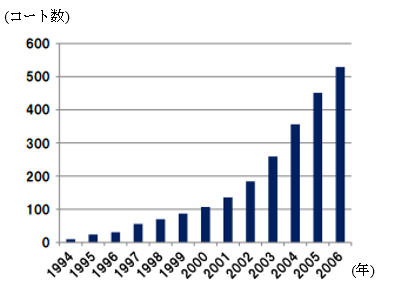
\includegraphics[width=85mm, bb=0 0 330 272]{figures/court.jpg}
	\caption{データ引用元 {\itshape レジャー白書2007}}
	\label{レジャー白書2007}
\end{figure}

フットサルプレイヤーの数はやや鈍化傾向にあるが、未だに緩やかな右肩上がりの成長を続けていると言える。
現在では、フットサルのプロリーグであるFリーグをはじめ、全国リーグ、公式戦・地方トーナメント・芸能人リーグの開催と共に、着実に競技人口を増やしつつある。

\begin{figure}[htbp]
	\centering
	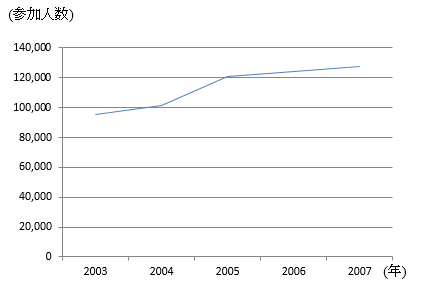
\includegraphics[width=85mm, bb=0 0 330 272]{figures/pati.jpg}
	\caption{データ引用元 {\itshape www.salon20002.net/monthly/2008/2008-22.pdf}}
	\label{www.salon20002.net/monthly/2008/2008-22.pdf}
\end{figure}

このように年々、フットサルコートは増えているが、フットサルプレイヤーの数は増えていない。特に東京郊外のフットサルコートのレンタルだけでは、運営が難しいので、フットサルスクールや大会を開催し、運営しているコートが多々ある。

\section{フラッシュマーケティングを用いた集客の取り組み}
次の章で詳細を述べるが、フラッシュマーケティング市場においてレクリエーションカテゴリが占める売上の割合は10%程であり、特にフットサルコートを始め、会員制クラブでもフラッシュマーケティングサイトが占める割合は少ない。ここでは、フットサルコートでフラッシュマーケティングが適用された事例を見ていく。

\subsection{LaBOLAクーポン}
 株式会社ラクシーズは2010年12月6日より、スポーツ・レジャーに特化した事前購入型クーポンサービス「LaBOLAクーポン」を開始し、フラッシュマーケティングに参入した。
LaBOLAクーポンとは、スポーツ・レジャーに特化したプレミアムクーポンを購入できるサービスであり、フットサルおよびサッカー情報提供サービスサイトを運営するラクシーズが運営しているスポーツSNS「LaBOLA(ラボーラ)」との連携による相乗効果を狙った。LaBOLAの会員数は2010年当時約10万人超。月間アクセス数 約300万PV。ユニークユーザー数は約50万人に及んでおり、既に会員を有しているコミュニティーとの連携は大きなアドバンテージと考えられていた。
\\ しかし2011年9月30日をもってサービスは終了している。元々フットサル、サッカーに特化したSNSのLaBOLAの顧客に対し、ヨガやゴルフ教室といったクーポンを提供していたことが、既存の顧客に対しての興味関心の相違がサービスの売上が伸び悩んだことの要因と考えられる。
\newpage

\subsection{Grouponにおけるレジャー施設の活用方法}
2010年から日本国内でサービスを始めたGrouponは、フットサルコートのクーポンの販売もしている。2012年まではコートのクーポンを販売していたが、近年では図にあるようにコートの使用だけではなく有名人をと一緒にフットサルを楽しめるイベント型のクーポンも販売している。都内のフットサルコートでは、イベント型のクーポンが増えている。
\\ 次の小節で詳しくフットサルコートがフラッシュマーケティングを取り入れない理由を述べるが、このようにクーポン自体に使用以外に他の特典を付けた理由は、フットサルコートのオーナーの調査を行った結果、以下二点が考えられる。
\\・利用者がクーポン購入後の使い方がよくわからない
\\・空きコートを掲載できるのが一日だけなので、購入されなえればそのまま空きコートのなる可能性が高い
\\
\\
\\
\\
\\
\\
\\
\begin{figure}[htbp]
	\centering
	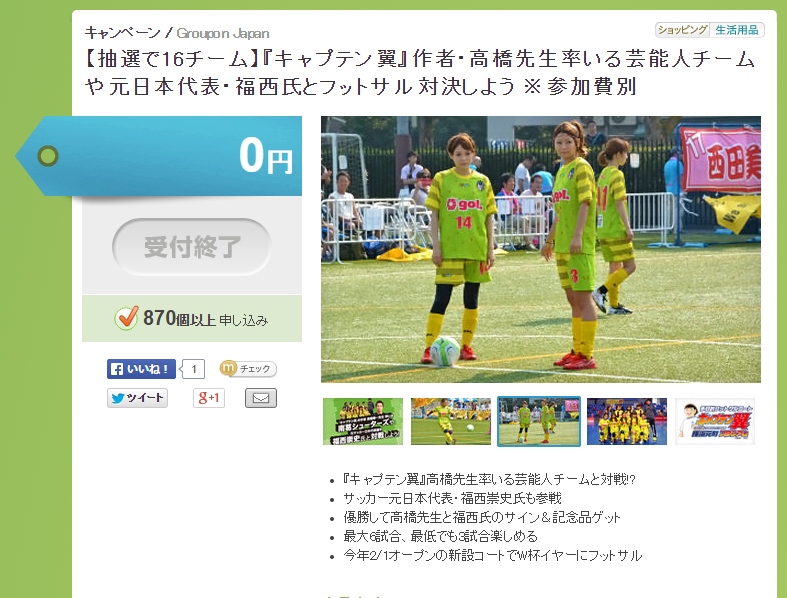
\includegraphics[width=85mm, bb=0 0 400 272]{figures/cap.jpg}
	\caption{データ引用元 {\itshape http://www.groupon.jp/cid/103608}}
	\label{www.salon20002.net/monthly/2008/2008-22.pdf}
\end{figure}


\section{問題提起}
上記のように、レクリエーション分野、特にフットサルコートにおいて、フラッシュマーケティングは上手く活用できているとは言えない。
そこで筆者は八王子、多摩地区所在する5つのフットサルコートのオーナーと首都圏を中心にフットサルコートを運営するエリアマネージャーにインタビュー調査を行い、フラッシュマーケティングの問題点とフラッシュマーケティングを用いらない理由を調査した。

\begin{itemize}
	\item 利用者がクーポン購入後の使い方がよくわからない
	\item 空きコートを掲載しても、購入されなえればそのまま空きコートのなる可能性が高い
	\item クーポンを出稿する際の文言を考えたり、手間がかかること。
	\item そもそもフラッシュマーケティングサイトに出稿されていることをフットサルプレイヤーはしらない
	\item ターゲット対象が、ある程度練習頻度が多いチームでないといけない
	\item そもそもクーポン購入客専用の対応を作らなければいけない
\end{itemize}



チーム人数が少ないフットサルチーム複数に対して、格安でフットサルコートを提供することで、コート運営者側はアイドリングの時間を削減することができ下記の問題を解決できると考えた。
\\・チーム人数の少ないチームはクーポンを買うことができない
\\・マッチング後の試合の運営方法
\\・コートの価格が高すぎる
\\・コートの集金リスクを軽減する

\section{実証と検証}
フラッシュマーケティングサイトにおけるビジネスモデルの変化、現在のレジャー施設、ユーザーにフラッシュマーケティングサイトの意識調査を行い、フラッシュマーケティングサイトの実態と照らし合わせた。その結果、購入する際のユーザー側の問題、フットサルコート側の集金リスクが課題であることが分かった。この問題を解決するために、フラッシュマーケティングサイトを構築し、ユーザー間のマッチングを図り、当サイトがフットサルコートの代わりに集金を担い実証実験を行った。
\section{本論の構成}
%\makeendnotes  %フットノートをすべて章末に移動するスクリプトです。使用しない場合はコメントアウトしてください。
本論の構成はまず1章で現状のレジャー施設の現状分析を行った後に、2章でフラッシュマーケティングに関する先行研究を述べ、本サービスに必要部分を抽出する。3章ではプロトタイプを用いり、ユーザーテストを行った。4章ではユーザーテスト時のユーザーのコメントを基に、サービスコンセプトを決めた。プロトタイプを修正したものを実際にサービスとして、各フットサルコートと提携し、運営内容を述べる。6章ではサービスの評価を行い、7章で結論を述べる。


%改ページしたい場合
%\newpage

%%%%%Notes%%%%%
%エンドノートを使用しない場合は以下をコメントアウトしてください。
\section*{注}
\addcontentsline{toc}{section}{注}
\begin{footnotesize}
%\theendnotes
\end{footnotesize}

